%%%%%%%%%%%%%%%%%%%%%%%%%%%%%%%%%%%%%%%%%%%%%%%%%%%%%%%%%%%%%%%%%%%%%%%%%%%%%%%%
%%%%%%%%%%%%%%%%%%%%%%%%%%%%%%%%%%%%%%%%%%%%%%%%%%%%%%%%%%%%%%%%%%%%%%%%%%%%%%%%
\section{\textcolor{blue}{Contagens dos passos para o ensino}}
Antes de iniciar esta seção é importante mencionar uma
problemática que é vista com muita frequência nas escolas de dança; 
esta é gerada devido a que: A forma em que os tempos são contados 
na música, é
diferente à realizada entre profissionais da música e da dança. 
Sendo que a contagem dos profissionais da música segue a \hyperref[def:Metrica]{\textbf{métrica}} indicada na partitura,
e no caso de profissionais da dança segue geralmente um enfoque 
particular a cada escola de dança, visando só em muitos casos o fácil entendimento do aluno da
execução do movimento programado para essa aula, e não uma rigorosidade teórica no uso de termos e 
expressões musicais.




\subsection{Contagem de 3 passos em 2 tempos}
Esta diferença na forma de perceber o inicio e o final do ciclo de repetição,
vista na Seção \ref{sec:percepcaoouvinte}, 
leva a um problema quando se quer ser rigoroso na forma de contar os tempos nos compassos; 
por exemplo, na Tabela \ref{tab:ritmo1} 
podemos ver 4 formas distintas, que podem adotar as pessoas, 
para contar os tempos nos compassos indicando a distribuição de tempos, 
onde ``$T$'' representa um tempo do compasso.
\begin{table}[ht]
  \centering
  \begin{tabular}    {c|ccc|c}
    \hline
    Tipos de contagem       & $T/2$ & $T/2$   & $T$ (Forte) & Recomendável?\\
    \hline
    Contagem 1: & tchic  & tchic  & tum   & Sim\\
    Contagem 2: & 2     & e     & 1     & Sim\\ \hline
    Contagem 3: & Con   & tra  & Tempo & Não\\
    Contagem 4: & 1     & e     & 2     & Não\\  \hline
    Contagem 5: & 1     & 2     & 3     & Depende\\ \hline
    \hline
  \end{tabular}
  \caption{Tipos de contagem na samba de gafieira.}
\label{tab:ritmo1}
\end{table}

As formas de contagem que recomendo são:
\begin{itemize}
\item \textbf{A contagem 1}, 
devido que a principio, pode ser usada sem aprofundar demasiado 
na notação musical, de modo que só precisa ser explicado que a duração de um 
``tum'' é o dobro que um ``tchic'', e anexar que tipicamente veremos que o ``tum''
acontece no tempo 1 do compasso; 
%de modo que outra contagem valida seria ``tum tchic tchic''; 
porem, a contagem 1 não está restrita ao uso destas silabas (``tchic'' e ``tum''), 
em geral esta contagem representa a quase qualquer padrão de repetição
que use duas silabas diferentes, como por exemplo os padrões: ``ta-ta kum'', ``tic-tic kum'', etc. 
Este tipo de contagem já é muito usada na pratica e na literatura, pois 
podemos achar variantes como ``quick-quick slow'' (rápido-rápido lento no idioma inglês)
ou ``tic-tic tum'' seguindo a notação usada por Perna no seu livro sobre samba de gafieira \cite[pp. 146]{perna2002samba}.
\item \textbf{A contagem 2}, segue a notação de tempos na partitura, este tipo de
contagem é coerente com a musica, porem precisa de uma major explicação, 
para pessoas não iniciadas na musica e a dança. Porem, isto não quer dizer que seu
entendimento seja complexo, e sim que precisa um investimento em horas de aula
um pouco major que a contagem 1.
Mesmo assim, devemos ter cuidado pois pode-se dar o caso que a partitura não tenha compassos binários 
e sim quaternários, com contagens ``2 e 3'' ``4 e 1'', 
criando este tipo de contagem mais caminhos onde podemos perder coerência com a contagem na partitura.\\
\end{itemize}


Entre as contagens que não recomendo estão:
\begin{itemize}
\item \textbf{A contagem 3} (``con-tra tempo''), 
devido a que o uso deste padrão pode confundir às pessoas que desconhecem 
a definição formal do termo contratempo \cite[pp. 16]{mascarenhascurso} \cite[pp. 36]{azevedocompor}, 
e levar a confusão de achar que um contratempo é só uma distribuição de 3 tempos, 
sendo um o dobro dos outros dois, em termos de tempos execução.
\item \textbf{A contagem 4} é não recomendada, devido a que como é visto nas Figuras 
\ref{fig:abc-caquarela} e \ref{fig:abc-contratempo1}, musicalmente a contagem estaria invertida,
dado que tipicamente o ``tum'' se execute no tempo 1.\\
\end{itemize}

Finalmente, a contagem que precisa um cuidado especial:
\begin{itemize}

\item \textbf{A contagem 5} precisa ser bem explicada, 
devido a que não segue a notação musical; 
porem, seu uso é didático e pode ser resgatado,
se fazemos em todo instante uma aclaração, 
que se trata de \hyperref[sec:TemposCoreograficos]{\textbf{tempos coreográficos}}.
Assim, ficara claro para o estudante, que estes não correspondem necessariamente, 
com os tempos musicais que também devem ser ensinados.
Para mais detalhes sobre os tempos coreográficos ver a Seção \ref{sec:TemposCoreograficos}.

%não é recomendada, 
%por motivos similares aos apresentados para a contagem 4. 
%Além do fato que os números atribuídos estão distantes da
%notação verdadeira na partitura, mesmo sim esta houvesse sido escrita num compasso quaternário.
\end{itemize}

\subsection{\textcolor{red}{Contagem de 2 passos em 2 tempos}}


Tabela \ref{tab:ritmoconta2}

\begin{table}[ht]
  \centering
  \begin{tabular}    {c|cc|c}
    \hline
    Tipos de contagem       & $T$ (fraco)  & $T$ (Forte)& Recomendável?\\
    \hline
    Contagem 1: & tum  & TUM  & Sim\\
    Contagem 2: & 2     & 1     & Sim\\
    Contagem 3: & tempo & Tempo & Sim\\ \hline
    Contagem 4: & 1     & 2     & Não\\ \hline
    Contagem 5: & 1     & 3     & Depende\\  \hline
    \hline
  \end{tabular}
  \caption{Tipos de contagem na samba de gafieira.}
\label{tab:ritmoconta2}
\end{table}

Para mais detalhes sobre os tempos coreográficos ver a Seção \ref{sec:TemposCoreograficos}.


%%%%%%%%%%%%%%%%%%%%%%%%%%%%%%%%%%%%%%%%%%%%%%%%%%%%%%%%%%%%%%%%%%%%%%%%%%%%%%%%
%%%%%%%%%%%%%%%%%%%%%%%%%%%%%%%%%%%%%%%%%%%%%%%%%%%%%%%%%%%%%%%%%%%%%%%%%%%%%%%%
\section{\textcolor{blue}{Contagem de tempos correográficos}}
\label{sec:TemposCoreograficos}
\index{Musicalidade!Tempos coreográficos}

falar da possibilidade de contar 123 567 sim se usa um nome diferente a contagem de tempo musical,
exemplo, tempos coreográficos

Ver Figura \ref{fig:contagemtempocoreografico}.
\begin{figure}
    \centering
    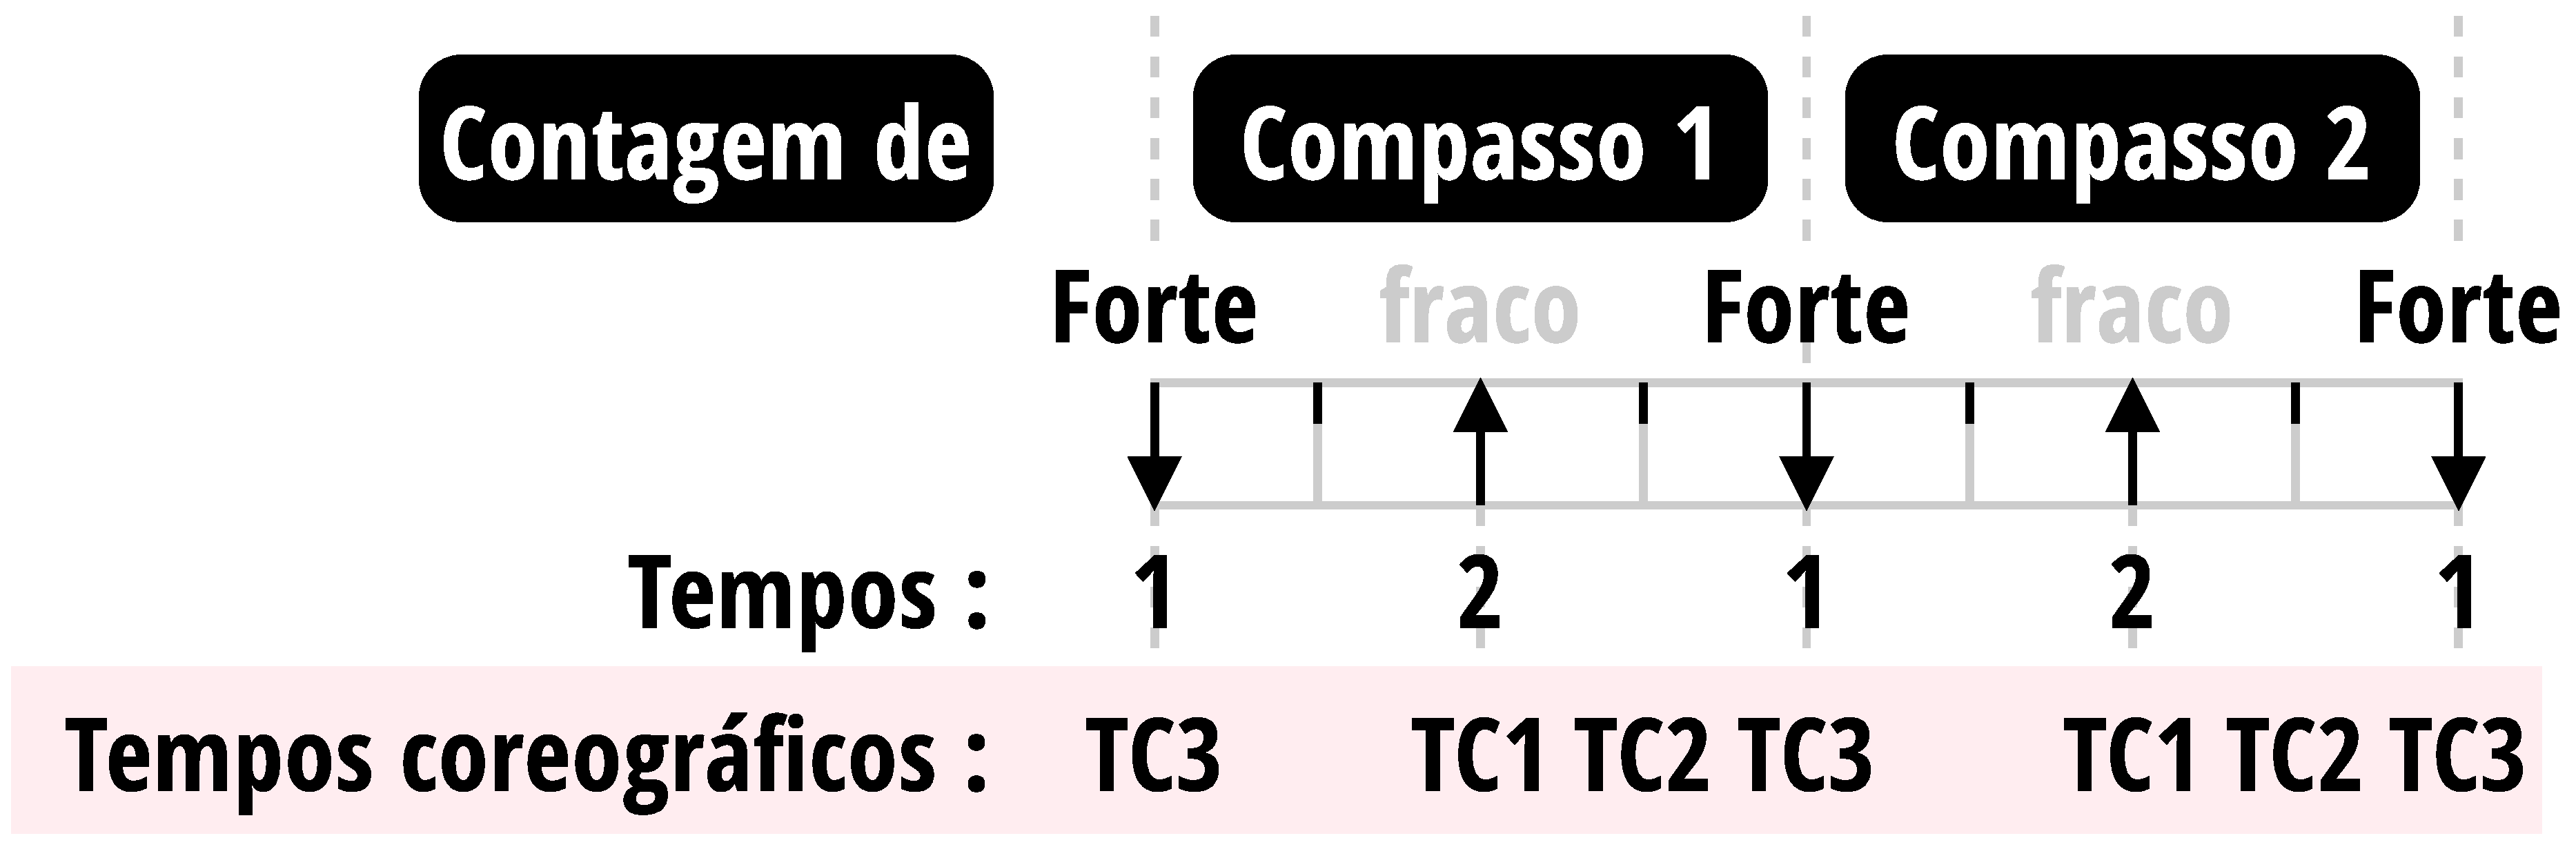
\includegraphics[width=\textwidth]{chapters/cap-musicalidade/contagemtempocoreografico.eps}
    \caption{Contando tempos coreograficos.}
    \label{fig:contagemtempocoreografico}
\end{figure}

